%!TEX TS-program = xelatex
%!TEX encoding = UTF-8 Unicode
%!BIB TS-program = biber
%!BIB program = biber

\documentclass[a4paper,11pt,twoside]{scrbook}

\usepackage[spanish]{babel}
\usepackage{xltxtra}
\usepackage{fontspec}
\usepackage{xunicode}
\usepackage{amsmath}
\usepackage{amsthm}
\usepackage[top=3cm,bottom=3cm,outer=3cm,inner=2cm]{geometry}
\usepackage[Bjornstrup]{fncychap}
\usepackage{graphicx}
\usepackage{amssymb}
\usepackage{hyperref}
\usepackage{enumerate}
\usepackage{siunitx}
\usepackage{float}
\usepackage{mdwlist}
\usepackage[table,usenames,dvipsnames]{xcolor}
\usepackage{titlesec}
\usepackage{subfigure}
\usepackage{csquotes}
\usepackage[style=authoryear,natbib=true,%
maxbibnames=99,maxcitenames=1,%
citestyle=authoryear-comp,doi=true,url=true,backend=biber,dashed=no]{biblatex}
\bibliography{\jobname}
\usepackage[hypcap]{caption}

\usepackage{makeidx}\makeindex
\usepackage{pifont}% http://tex.stackexchange.com/questions/42619/x-mark-to-match-checkmark
\newcommand{\cmark}{{\color{OliveGreen}\ding{51}}}
\newcommand{\xmark}{{\color{red}\ding{55}}}

%% plantuml %%
\usepackage{filecontents}
\usepackage{tikz}

\sisetup{output-decimal-marker={.},
	product-units=single,
	detect-all, detect-inline-family=text, detect-inline-weight=text,
  detect-display-math=true}

%% minted %%
\floatstyle{ruled}
\usepackage{minted}
\newcommand{\codep}[2][python]{%
	\mintinline{#1}{#2}%
}
\renewcommand{\listingscaption}{Código}
\renewcommand{\listoflistingscaption}{Tabla de códigos}
\setminted{breaklines=true,linenos=true}

%% estilo %%

\setmonofont[Scale=0.7]{Menlo}
\newfontfamily\portadafont{Arial Bold}


\begin{document}

\frontmatter

\pagenumbering{gobble}
\clearpage
%!TEX root = pfc-memoria.tex
%!TEX encoding = UTF-8 Unicode

\thispagestyle{empty}

\begingroup

\begin{center}
\includegraphics[width=4cm]{logo-us}\\[1.3cm]

\Large

\portadafont

ESCUELA TÉCNICA SUPERIOR DE INGENIERÍA INFORMÁTICA\\[0.8cm]

INGENIERO EN INFORMÁTICA (Plan 97)\\[2.8cm]

\MakeUppercase{\pfctitle}\\[2.7cm]

\large

Realizado por\\[0.1cm]

\MakeUppercase{\pfcauthor}\\[0.8cm]

Dirigido por\\[0.1cm]

JOSÉ ANTONIO TROYANO\\[0.8cm]

Departamento\\[0.1cm]

LENGUAJES Y SISTEMAS INFORMÁTICOS\\[3.6cm]


\end{center}

\begin{flushright}
\portadafont
Sevilla, \pfcdate
\end{flushright}

\endgroup


\cleardoublepage
\pagenumbering{arabic}
\tableofcontents

\mainmatter

%% %% %% %% %% %% %%

%!TEX root = pfc-memoria.tex
%!TEX encoding = UTF-8 Unicode

\cleardoubleevenemptypage
\part{Introducción y objetivos}
\label{part:introduccion-objetivos}

%!TEX root = pfc-memoria.tex
%!TEX encoding = UTF-8 Unicode

\chapter{Introducción}



%!TEX root = pfc-memoria.tex
%!TEX encoding = UTF-8 Unicode

\chapter{Planificación}

\epigraph{``El progreso no se consigue por la suerte o por accidente sino trabajando en uno mismo diariamente.''}{\textsc{Epictetus} (55--135)}

En este capítulo organizaremos el desglose de tareas para hacer una planificación de las mismas en el calendario.

\section{Metodología de trabajo}

Utilizaremos un modelo de ciclo de vida iterativo en espiral \citep{Boehm1988}, pero dividiendo el proceso en dos paquetes de trabajo:
\begin{enumerate}[WP1]
\item La lectura y estudio de la bibliografía sobre NLP y ML; y su parte de documentación en la memoria.
\item Estudio de bibliotecas y frameworks disponibles para la construcción del GUI; y análisis, diseño, implementación y pruebas del software; y su parte de documentación en la memoria.
\end{enumerate}

\begin{figure}[htbp]
\centering
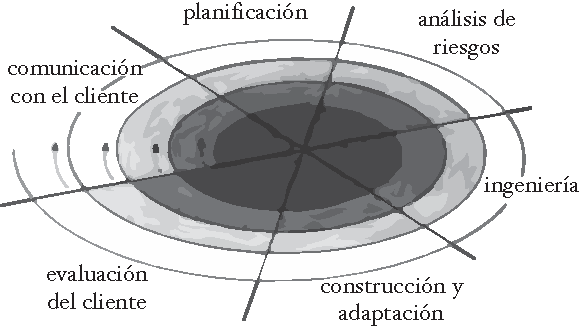
\includegraphics[width=0.58\textwidth]{espiral}
\caption[Modelo de ciclo de vida en espiral]{Modelo de ciclo de vida en espiral \citep{Boehm1988}}
\label{fig:espiral}
\end{figure}

El tutor de proyecto, que hace de cliente, recibió aproximadamente una comunicación cada semana y media o dos semanas, durante junio y julio, con el progreso de la memoria por capítulos.

\section{Herramientas utilizadas}

Para la elaboración de la memoria, utilizamos el sistema de composición tipográfica \XeLaTeX. Para el retoque de imágenes, y de ilustraciones: Adobe Photoshop y Adobe Illustrator. Para la gestión bibliográfica usamos la aplicación Mendeley.

Para generar los diagramas en UML, casos de uso, clases, etc. usamos el intérprete PlantUML\footnote{\url{http://www.plantuml.com/}} que se apoya en el motor de rendering Graphviz.\footnote{\url{http://www.graphviz.org/}}

Como gestor de código fuente: \codet{git} en local, y el servicio de Bitbucket\footnote{\url{https://bitbucket.org}} como respaldo.

Para la codificación en Python, usamos el IDE de Jetbrains PyCharm.

\section{Planificación y coste}

El desglose de tareas se puede ver en la \autoref{tbl:tareas}. Para el cálculo, se ha estimado un día de trabajo de 8 horas, y una semana de 5 días, de lunes a viernes. Se estimó inicialmente un esfuerzo necesario de \framebox[2cm]{14w~0d~1h}, al que hay que sumar un retraso de \framebox[2cm]{1w~3d~0h} por los problemas con el framework Kivi~1.9, y en la implementación de la tabla de datos en QML. Estos dos problemas se comentarán más adelante en el \fullref{chap:implementacion}.

Por lo tanto, se ha realizado un trabajo final de \SI{625}{horas}, aunque lo estimado fueron \SI{561}{horas}. Suponiendo un precio presupuestado de \SI{9.5}{€/hora}:
\[
\SI{561}{horas} \times \SI{9.5}{€/hora} \; = \; \SI{5329.5}{€} 
\]

\begin{table}[htbp]
\centering
\csvautotabular{gantt.csv}
\caption{Listado de tareas del proyecto}
\label{tbl:tareas}
\end{table}

%Se puede ver un diagrama de Gantt con el calendario de las tareas en las figuras \ref{fig:gantt1} y \ref{fig:gantt2}.

En la página \pageref{fig:gantt} se muestra el diagrama de Gantt con el calendario de las tareas.

\FloatBarrier

%\begin{landscape}
\includepdf[landscape=true,pagecommand={\thispagestyle{empty}\begin{figure}[H]\caption[Cronograma (diagrama de Gantt)]{}\label{fig:gantt}\end{figure}}]{gantt.pdf}
%\end{landscape}

%\begin{landscape}
%\begin{figure}[htbp]
%\centering
%\vspace*{0.6cm}
%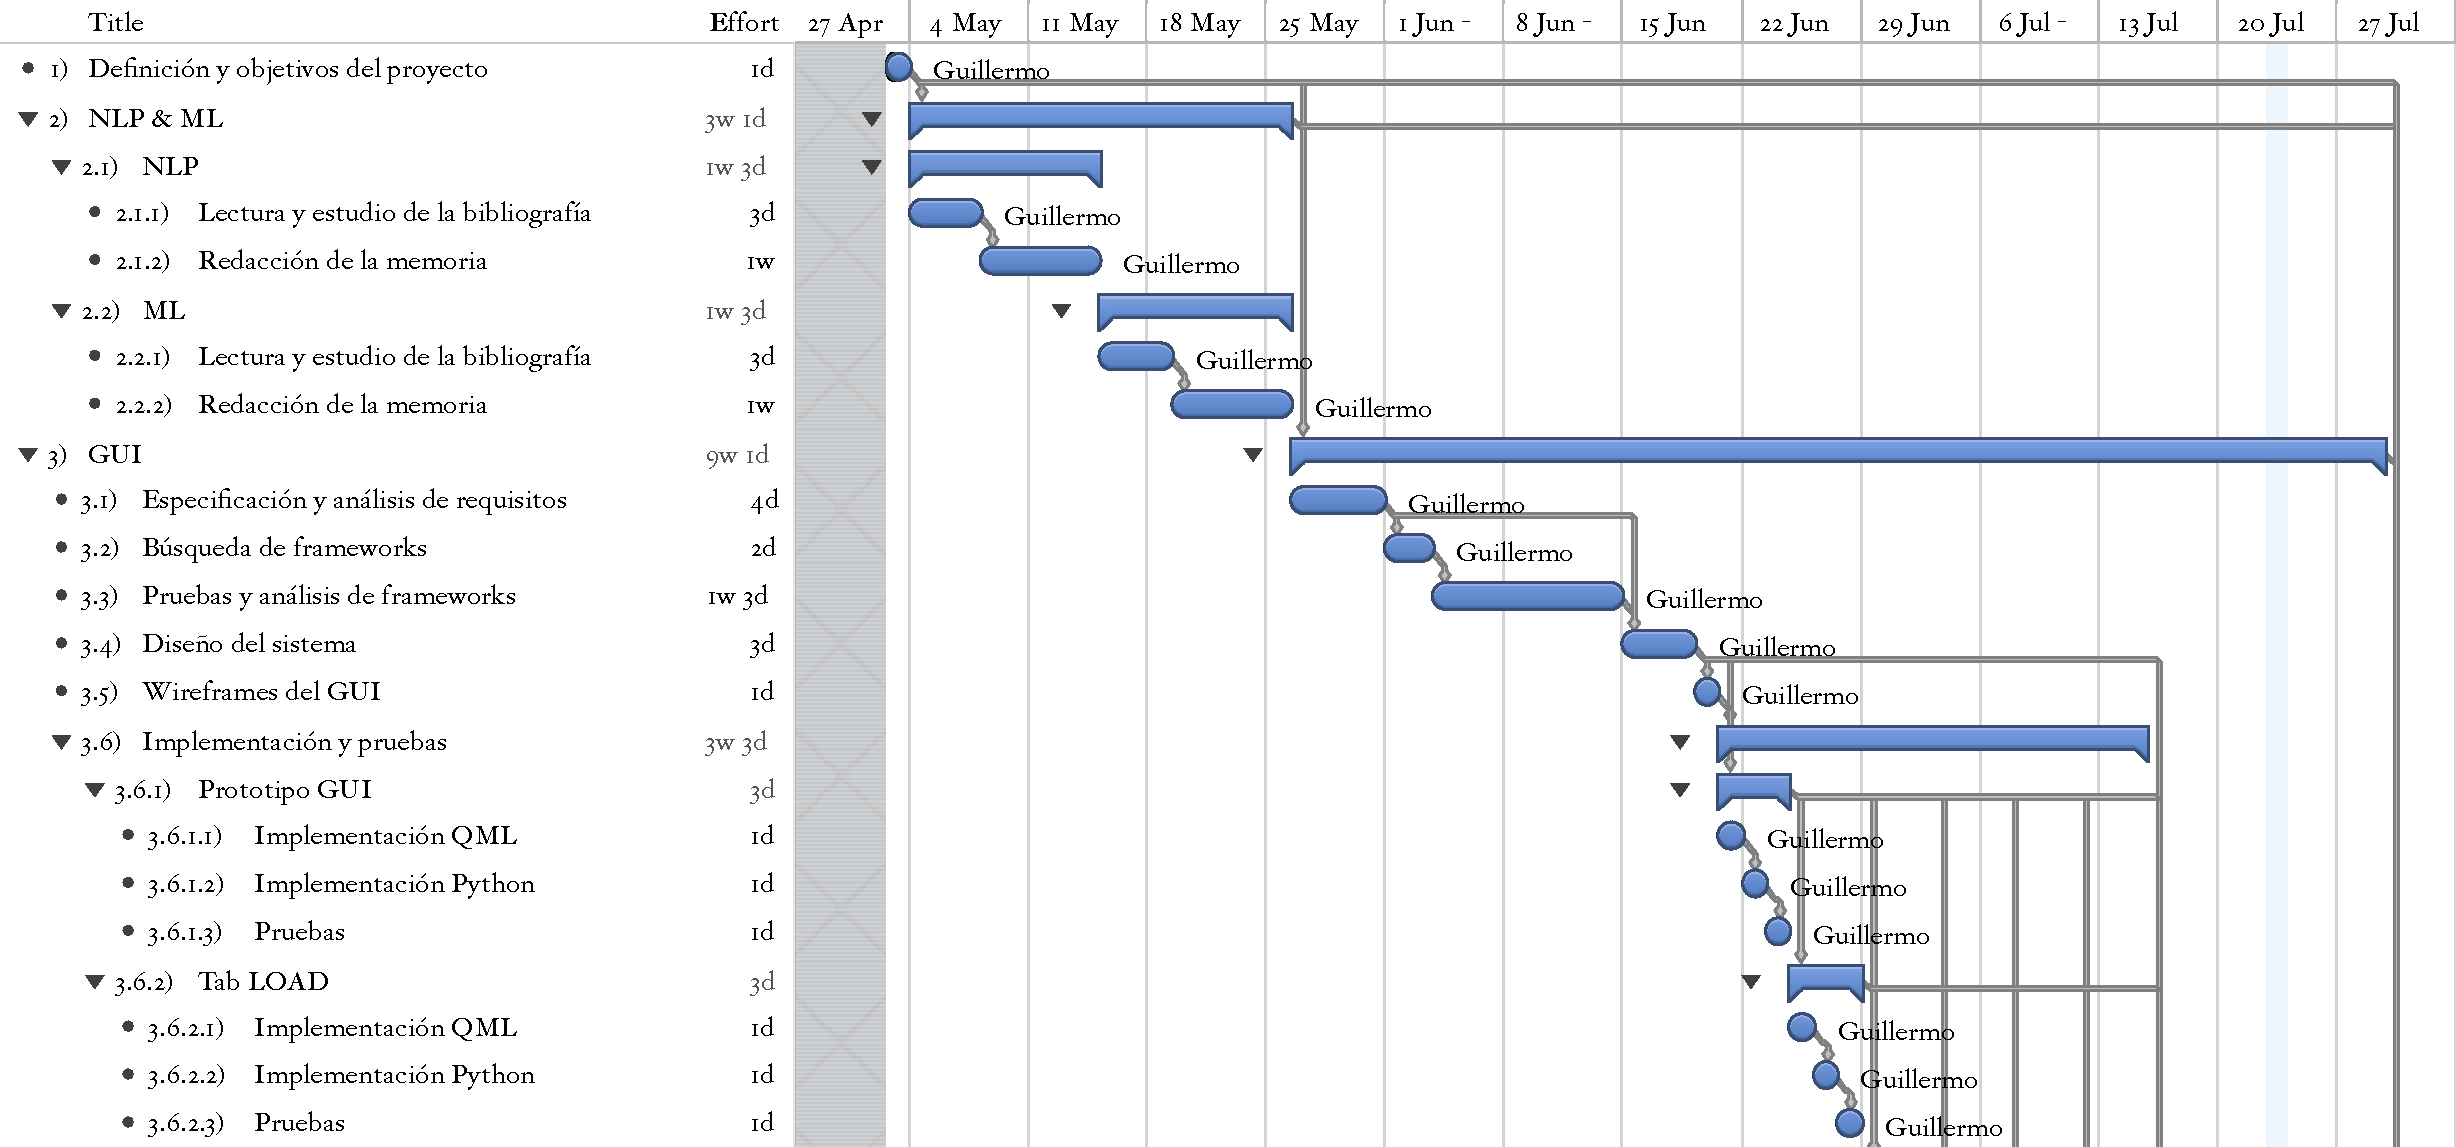
\includegraphics[width=24cm]{gantt1.pdf}
%\caption{Cronograma (I)}
%\label{fig:gantt1}
%\end{figure}
%\end{landscape}
%
%\begin{landscape}
%\begin{figure}[htbp]
%\todo{pendiente corregir la calidad de este segundo corte del diagrama}
%\centering
%\vspace*{0.6cm}
%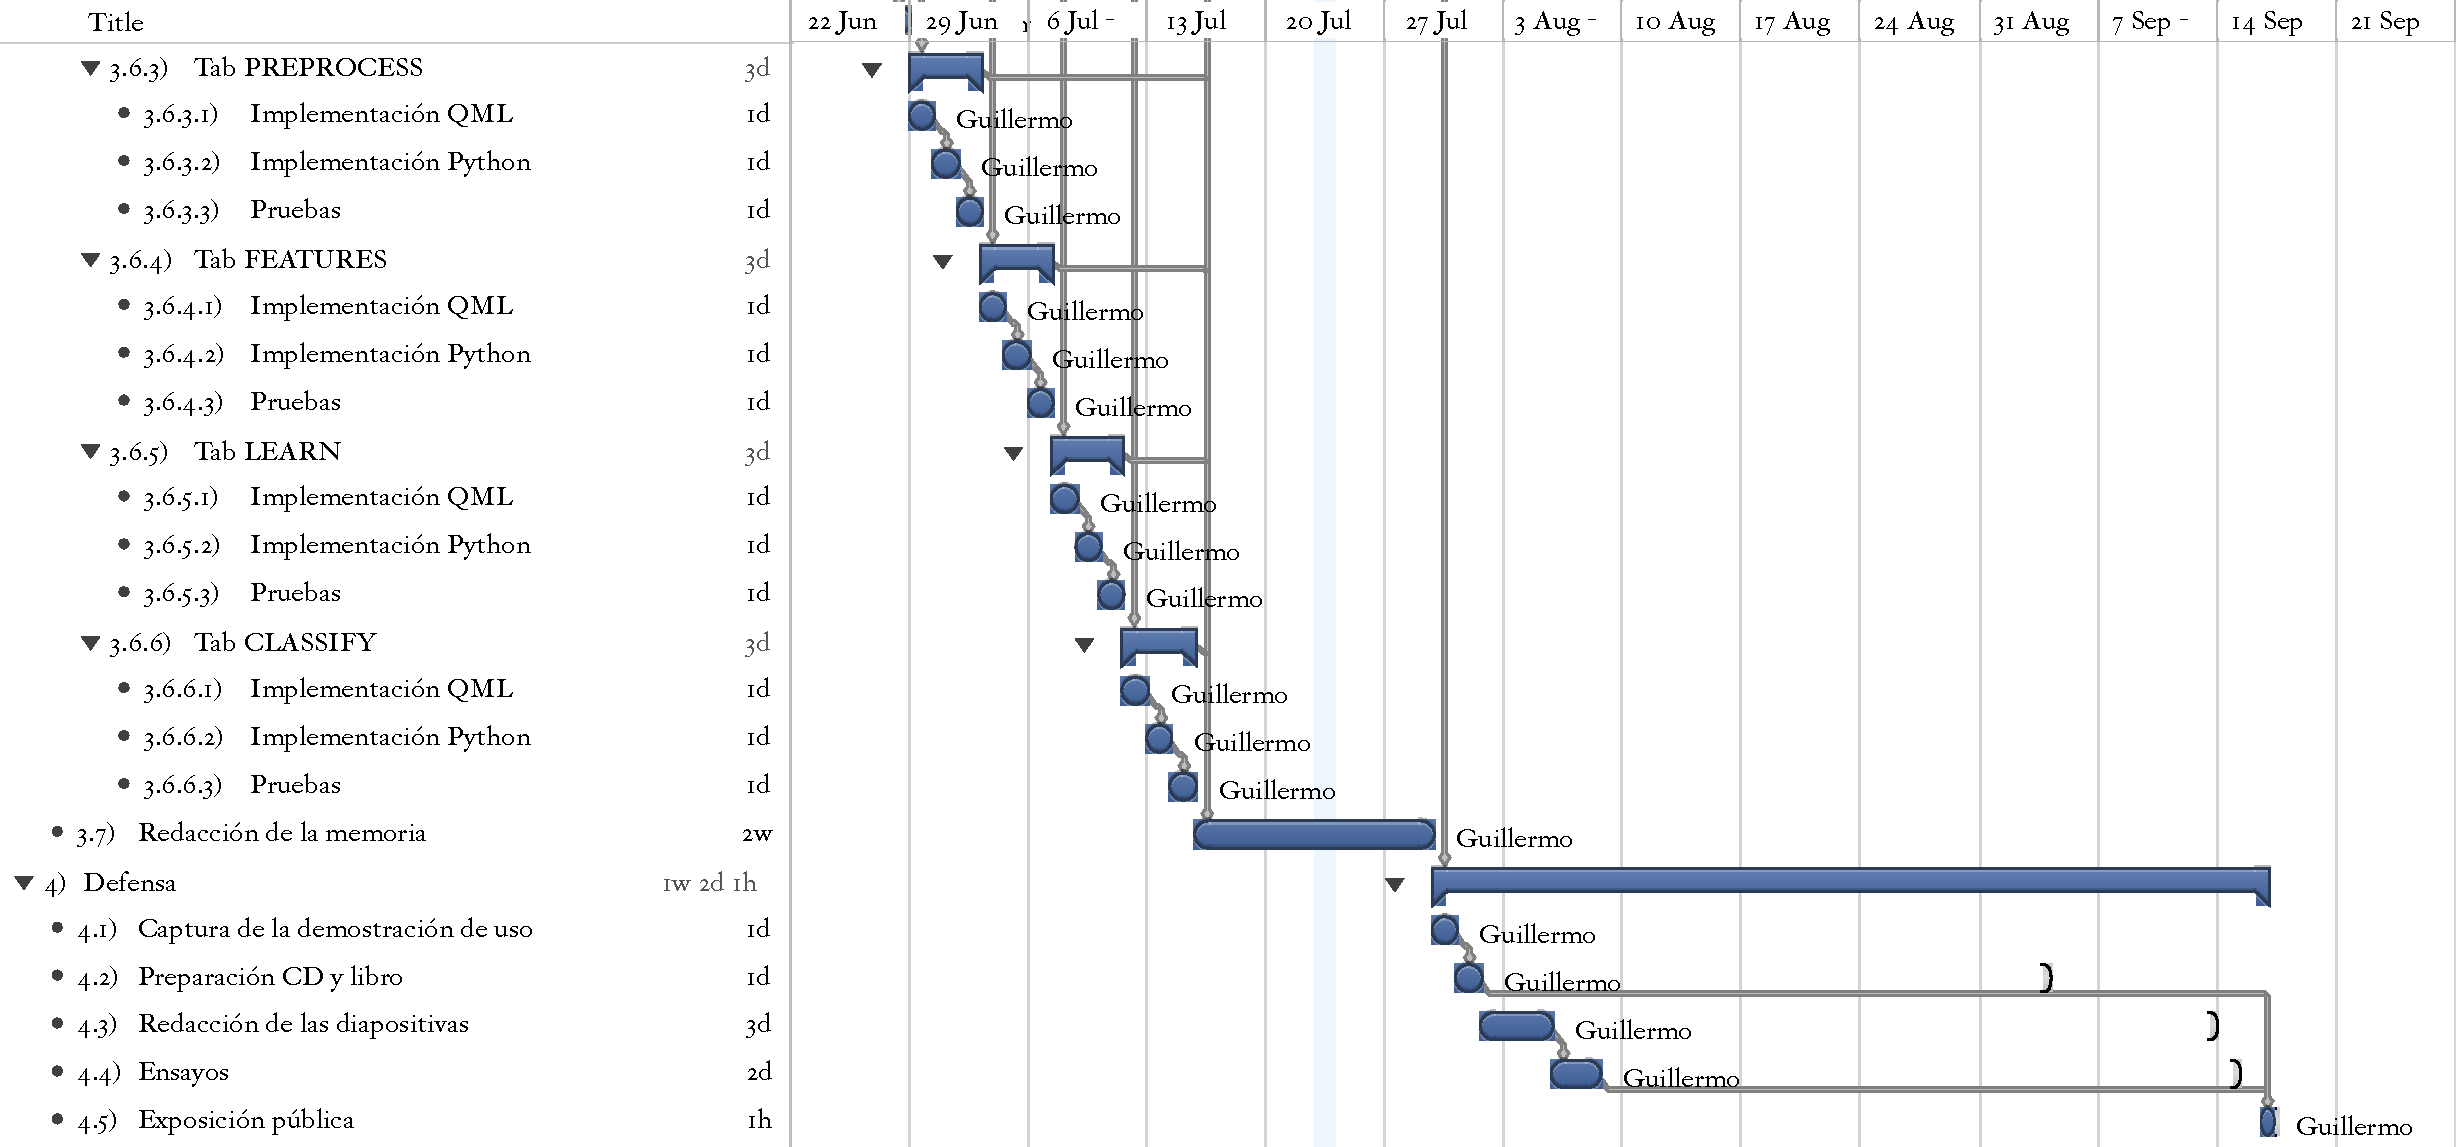
\includegraphics[width=24cm]{gantt2b.pdf}
%\caption{Cronograma (y II)}
%\label{fig:gantt2}
%\end{figure}
%\end{landscape}



\cleardoubleevenemptypage
\part{Investigación y estudio}
\label{part:investigacion-estudio}

%!TEX root = pfc-memoria.tex
%!TEX encoding = UTF-8 Unicode

\chapter{Procesamiento del Lenguaje Natural}

\section{Preprocesamiento}

\subsection{\emph{``Tokenización''}}

La \emph{tokenización}\index{tokenización}\index{tokenization@\emph{tokenization}} en NLP es normalmente el proceso de separar la cadena de entrada, frases en lenguaje natural, en las distintas palabras que componen la frase. Puede ser simplemente un separador que trocee la frase cada vez que se encuentre un espacio.
\begin{listing}[H]
\begin{minted}{python}
>>> 'of escapades demonstrating the adage that what is good for the goose'.split()
['of', 'escapades', 'demonstrating', 'the', 'adage', 'that', 'what', 'is', 'good', 'for', 'the', 'goose']
>>> 
\end{minted}
\caption{Tokenización sencilla mediante la separación de espacios.}
\label{lst:tokenizacion-sencilla}
\end{listing}

La tokenización en su sentido más amplio y general es el procedimiento del análisis léxico para reconocer lexemas del flujo de entrada con la que se obtiene un flujo de salida compuesto por tokens \citep[§2.2]{Jimenez2004}.

\begin{definition}[Token] \index{token}
Denominamos \emph{token} al conjunto de cadenas de caracteres con significado mínimo.
\end{definition}

\begin{definition}[Patrón] \index{patrón}
El \emph{patrón} es una regla que describe el conjunto de caracteres que cuadran un token.
\end{definition}

El concepto de ``cuadrar'' se denomina en inglés como match\index{match@\emph{match}}, y también se puede traducir como concordancia o correspondencia.

\begin{definition}[Lexema] \index{lexema}
Un \emph{lexema} es una secuencia concreta de caracteres que se corresponde con el patrón de un token determinado.
\end{definition}

\begin{example} \index{token} \index{patrón} \index{lexema}
Pongamos algunos ejemplos de tokens, patrones y lexemas, de un lenguaje formal típico de programación:
\nopagebreak
\begin{center}
\begin{tabular}{|l|l|l|}
\hline
\textbf{token} & \textbf{lexemas de ejemplo} & \textbf{descripción informal del patrón} \\ \hhline{===}
\codep{CONST} & \codep{const} & const \\ \hline
\codep{IF} & \codep{if} & if \\ \hline
\codep{OPREL} & \codep{<}, \codep{<=}, \codep{=}, \codep{>}, \codep{>=} & <~ ó <= ó = ó >~ ó >= \\ \hline
\codep{ID} & \codep{pi}, \codep{contador}, \codep{D2} & letra seguida de letras y dígitos \\ \hline
\codep{CTENUM} & \codep{3.1416}, \codep{0}, \codep{6.1E23} & cualquier constante numérica \\ \hline
\codep{LITERAL} & \codep{"core dumped"} & cualesquiera letras entre \codep{"} y \codep{"} excepto \codep{"} \\ \hline
\end{tabular}
\end{center}
\end{example}

En lenguaje natural, la unidad mínima de información textual será la palabra. De manera que token y lexema coinciden siempre, y no tiene sentido definir un patrón para cada token de las palabras de un diccionario de la lengua, ya que el patrón es la propia secuencia de letras de la palabra.

Existen distintos niveles de tokenización de documentos \citep[ch.~1]{Perkins2010}:
\nopagebreak
\begin{itemize}
\item Tokenizar textos en frases.
\item Tokenizar frases en palabras.
\end{itemize}

Simplemente para la primera tarea ya nos encontramos con dificultades, pues las frases no sólo terminan en punto. Pueden terminar en punto (\codep{.}), signo de exclamación (\codep[text]{!}), signo de interrogación (\codep[text]{?}), en algunos casos dos puntos (\codep{:}). Y en otros idiomas, como el español, también hay que tener en cuenta que en la separación entre frases puede haber signos de apertura de interrogación o exclamación, etc.

En cuanto a la separación de palabras, también pueden surgir problemas, dependiendo del idioma. En el siguiente ejemplo (\autoref{lst:wordtokenizers}) podemos ver distintas formas de separar palabras de una frase en inglés que usa contracciones.\footnote{También se puede encontrar un demostrador interactivo de la tokenización en la siguiente dirección:\\
\url{http://text-processing.com/demo/tokenize/}}

\begin{listing}[H]
\begin{minted}{python}
>>> from nltk.tokenize import TreebankWordTokenizer, WordPunctTokenizer, WhitespaceTokenizer
>>> TreebankWordTokenizer().tokenize("Can't is a contraction.")
['Ca', "n't", 'is', 'a', 'contraction', '.']
>>> WordPunctTokenizer().tokenize("Can't is a contraction.")
['Can', "'", 't', 'is', 'a', 'contraction', '.']
>>> WhitespaceTokenizer().tokenize("Can't is a contraction.")
["Can't", 'is', 'a', 'contraction.']
>>> 
\end{minted}
\caption{Diferentes estrategias de separación de palabras}
\label{lst:wordtokenizers}
\end{listing}

Una mejor aproximación al problema es reemplazar --previamente a la tokenización--, las palabras contraídas con sus palabras equivalentes sin contracción.\footnote{Puede obtenerse un catálogo bastante extenso de contracciones en inglés --en uso y arcaicas--, en la dirección: \url{http://www.enchantedlearning.com/grammar/contractions/list.shtml}}
Para ello es necesario construirse una tabla que establezca el mapping \citep{Perkins2014}.

Como ejemplo de un conjunto de substitución, véase una tabla no exhaustiva en la \autoref{tbl:contracciones}, en dos versiones:
\nopagebreak
\begin{enumerate}[(a)]
\item En la primera de ellas se implementaría empleando un diccionario común de palabras de búsqueda y reemplazo, directamente.
\item En la segunda opción, se hace uso de expresiones regulares para condensar la tabla y no tener que hacer explícito todas las posibles contracciones que compartan sufijos sinónimos.
\end{enumerate}

\begin{table}[htbp]
\centering
\begin{subtable}[t]{0.45\linewidth}
\centering
\begin{tabular}{|l|l|}
\hline
\textbf{contracción} & \textbf{reemplazar con} \\ \hhline{==}
isn't & is not \\ \hline
aren't & are not \\ \hline
wasn't & was not \\ \hline
weren't & were not \\ \hline
haven't & have not \\ \hline
hasn't & has not \\ \hline
couldn't & could not \\ \hline
shouldn't & should not \\ \hline
mightn't & might not \\ \hline
mustn't & must not \\ \hline
could've & could have \\ \hline
might've & might have \\ \hline
must've & must have \\ \hline
ma'am & madam \\ \hline
she'd've & she would have \\ \hline
'tisn't & it is not \\ \hline
who'll & who will \\ \hline
when'll & when will \\ \hline
what're & what are \\ \hline
we're & we are \\ \hline
they're & they are \\ \hline
that's & that is \\ \hline
I'll & I will \\ \hline
you'll & you will \\ \hline
he'll & he will \\ \hline
she'll & she will \\ \hline
\end{tabular}
\caption{Sustitución literal}
\label{tbl:contracciones-directa}
\end{subtable}
\begin{subtable}[t]{0.45\linewidth}
\centering
\begin{tabular}{|l|l|}
\hline
\textbf{contracción} & \textbf{reemplazar con} \\ \hhline{==}
\verb=r"won't"= & \verb="will not"= \\ \hline
\verb=r"can't"= & \verb="cannot"= \\ \hline
\verb=r"i'm"= & \verb="i am"= \\ \hline
\verb=r"ain't"= & \verb="is not"= \\ \hline
\verb=r"(\w+)'ll"= & \verb="\g<1> will"= \\ \hline
\verb=r"(\w+)n't"= & \verb="\g<1> not"= \\ \hline
\verb=r"(\w+)'ve"= & \verb="\g<1> have"= \\ \hline
\verb=r"(\w+)'s"= & \verb="\g<1> is"= \\ \hline
\verb=r"(\w+)'re"= & \verb="\g<1> are"= \\ \hline
\verb=r"(\w+)'d"= & \verb="\g<1> would"= \\ \hline
\end{tabular}
\caption{Sustitución condensada mediante expresiones regulares}
\label{tbl:contracciones-regexp}
\end{subtable}
\vfill
\caption{Sustitución de contracciones en inglés}
\label{tbl:contracciones}
\end{table}

\subsection{Supresión de palabras vacías (\emph{stopwords})}

\ldots

\subsection{Radicación \emph{``Stemming''}}

La \emph{decodificación primaria}\index{decodificación primaria} es la herramienta instintiva que permite a los hablantes de un idioma intuir el significado de una palabra desconocida del idioma --siendo conocido el subconjunto común y más frecuente del mismo--, a partir de sus elementos léxicos \citep{Zubira2002}. Son tres:
\nopagebreak
\begin{description}
\item[La contextualización.]\index{contextualización} Por medio de este mecanismo rastreamos el significado de la palabra valiéndonos del contexto o entorno de las frases en las cuales está inscrita. Ejemplos:
\nopagebreak
\begin{itemize}
\item ``Lo admiran por su \textbf{sindéresis}, ya que su \emph{capacidad para juzgar} es notable.'' $\Longrightarrow$ El contexto nos permite deducir que el significado de sindéresis es la capacidad para juzgar.
\item ``Los \emph{derechos económicos, sociales y culturales} son de segundo orden. Los \textbf{DESC} suponen mayores demandas.'' $\Longrightarrow$ El contexto nos permite intuir que el acrónimo DESC se refiere a derechos económicos, sociales y culturales.
\end{itemize}
%
\item[La sinonimia.]\index{sinonimia} Mediante la sinonimia, se puede hacer coincidir el significado de la palabra desconocida con términos semejantes que se han mencionado antes de ella (anáfora) o que se mencionarán después (catáfora) en el texto. Ejemplo:
\nopagebreak
\begin{itemize}
\item ``Nadie ha visto al \textbf{abate}. Parece que este \emph{clérigo} ha desaparecido.'' $\Longrightarrow$ El sinónimo de abate es clérigo, aunque seguramente tenga algún matiz que lo convierte en un término con mayor especificidad.
\end{itemize}
%
\item[La radicación.]\index{radicación} En inglés \emph{stemming}\index{stemming@\emph{stemming}}. La radicación consiste en descomponer la palabra en sus elementos constituyentes o afijos: prefijos, infijos y sufijos. Ejemplos:\footnote{Pueden consultarse más ejemplos en \url{http://www.slideshare.net/sandracasierra/decodificacin-primaria}}
\nopagebreak
\begin{itemize}
\item \textbf{postdiluviano} $\Longrightarrow$ Después (post-) de un diluvio.
\item \textbf{subtropical}  $\Longrightarrow$ Por debajo (sub-) del trópico.
\end{itemize}
\end{description}

La manera más común de realizar la radicación\index{radicación}\index{stemming@\emph{stemming}} en aplicaciones de NLP es eliminar los sufijos para quedarse con la raíz de la palabra, y su significado más primitivo (véase \autoref{lst:PorterStemmer}).

\begin{listing}[htbp]
\begin{minted}{python}
>>> from nltk.stem import PorterStemmer
>>> stemmer = PorterStemmer()
>>> stemmer.stem('cookery')
'cookeri'
>>> stemmer.stem('cooking')
'cook'
>>> stemmer.stem('series')
'seri'
>>> stemmer.stem('women')
'women'
>>> stemmer.stem('riding')
'ride'
>>> 
\end{minted}
\caption{Funcionamiento de \codep{PorterStemmer}}
\label{lst:PorterStemmer}
\end{listing}

\codep{PorterStemmer} es la implementación en NLTK del algoritmo de radicación de Martin Porter \citep{Porter1980}. Es un algoritmo --muy usado para lengua inglesa--, de eliminación o reemplazo de sufijos en varias iteraciones.

Aunque se pierda algo de información, tiene sus ventajas:
\nopagebreak
\begin{itemize}
\item Sirve para reducir el tamaño del vocabulario; y por consiguiente, el orden del tiempo y el espacio que ocupan los programas de procesamiento.
\item Sirve para asemejar conceptos similares, que es normalmente lo deseable al hacer una búsqueda o extracción de información.
\item También sirve para acelerar el procesamiento y reducir el tamaño de los índices de los motores de búsqueda.
\end{itemize}

No obstante también tiene alguna desventaja:
\nopagebreak
\begin{itemize}
\item Al estar basado en la eliminación literal de sufijos, puede producir palabras no válidas del idioma (como en \codep{'cookeri'} en el ejemplo anterior).
\end{itemize}

NLTK proporciona otros stemmers adicionales a \codep{PorterStemmer}:
\begin{description}
\item[\codep{LancasterStemmer}] Desarrollado en la Universidad de Lancaster, es ligeramente más agresivo que el algoritmo de Porter, aunque no existen estudios que confirmen la supremacía de uno sobre el otro \citep{Perkins2014}.
\item[\codep{RegexpStemmer}] Stemmer al que se puede recurrir para eliminar prefijos o sufijos de manera personalizada configurado mediante una expresión regular.
\item[\codep{SnowballStemmer}] Snowball extiende el método Porter para su aplicación a otros idiomas indoeuropeos: románicos, germánicos y escandinavos.
\end{description}

\subsection{Lematización}

La lematización\index{lematización} (\emph{lemmatizing}\index{lemmatizing@\emph{lemmatizing}} en inglés) es el proceso lingüístico que sustituye una palabra con forma \emph{flexionada} (plural, femenino, verbo conjugado, \ldots) por su \textbf{lema}. Tiene el mismo objetivo que la radicación, pero a diferencia de aquel, la lematización siempre produce una palabra válida en el idioma.
\begin{definition}[Lema]
En lingüística, el \emph{lema}\index{lema} es la forma que por convenio se acepta como representante de todas las formas flexionadas de una misma palabra.
\end{definition}

\subsection{Anotación gramatical de la parte de la oración (\emph{Part-of-speech tagging}) }

En gramática tradicional, la clasificación según categorías gramaticales es de tipo semántico y no funcional. En la gramática española el término fue introducido por Antonio de Nebrija \citep[Categoría gramatical]{wikipedia-es}. La gramática tradicional distingue nueve partes de la oración\index{parte de la oración}\index{part-of-speech\emph{part-of-speech}} (las ocho de Nebrija más el artículo):
\nopagebreak
\begin{enumerate}
\item Artículo o determinante
\item Sustantivo o nombre
\item Pronombre
\item Verbo
\item Adjetivo
\item Adverbio
\item Preposición
\item Conjunción
\item Interjección
\end{enumerate}

\chapter{Aprendizaje automático}

\section{Clasificadores}

\subsection{Bondad del clasificador (valor-F)}

Para la comparación de sistemas de búsqueda y recuperación de información disponemos de una métrica llamada valor-F\index{valor-F} (\emph{F-score}\index{F-score@\emph{F-score}}, \emph{F-measure}\index{F-measure@\emph{F-measure}} ó \emph{$F_1$ score}\index{F\_1 score@$F_1$ score}) siendo ésta la media armónica de otros dos indicadores \citep[Precisión y exhaustividad]{wikipedia-es}:
\begin{description}
\item[precisión \emph{(precision)}] \index{precisión}\index{precision@\emph{precision}}
Es la fracción de instancias recuperadas que son relevantes.
\begin{eqnarray}
\text{precisión} &=& \frac{|\{\text{relevantes}\}\cap\{\text{recuperados}\}|}{|\{\text{recuperados}\}|}
\end{eqnarray}
\item[exhaustividad \emph{(recall)}] \index{exhaustividad}\index{recall@\emph{recall}}
Es la fracción de instancias relevantes que han sido recuperadas.
\begin{eqnarray}
\text{exhaustividad} &=& \frac{|\{\text{relevantes}\}\cap\{\text{recuperados}\}|}{|\{\text{relevantes}\}|}
\end{eqnarray}
\item[valor-F \emph{(F-score)}] Media armónica de precisión y exhaustividad.
\begin{eqnarray}
F_1 &=& 2\times\frac{\text{precisión}\times\text{exhaustividad}}{\text{precisión}+\text{exhaustividad}}
\end{eqnarray}
\end{description}

Supongamos un clasificador binario:
\begin{itemize}
\item La medida de precisión será el porcentaje de documentos correctamente clasificados dentro del conjunto de prueba.
\item La medida de exhaustividad será el porcentaje de documentos del conjunto de referencia que han sido correctamente clasificados. \citep{Perkins2010}
\end{itemize}


\section{Rendimiento en Python}

Se observó que la carga del modelo entrenado \path{GoogleNews-vectors-negative300.bin.gz} consumía mucho tiempo y espacio ($\approx$\si{4.5}{GiB} y unos 5 minutos). Este modelo ha sido publicado por Google en el repositorio del proyecto \codep{word2vec} basado en el \emph{dataset} de Google News (aproximadamente 100 mil millones de palabras). El modelo contiene vectores 300-dimensionales para 3 millones de palabras y de frases (bigramas y trigramas). Las frases se obtuvieron usando una aproximación dirigida por datos sencilla, como se encuentra descrito en \cite{DBLP:journals/corr/MikolovSCCD13}.

Por ello se convirtió inicialmente el modelo del \emph{Word2Vec} original en la representación interna provista por \codep{gensim}, que soporta en \emph{unpickling} de datos de NumPy, de mejor desempeño.

El procedimiento para la conversión es:

\begin{listing}[H]
\begin{minted}{python}
from gensim.models.word2vec import Word2Vec
# lectura sin optimizar
model_orig = Word2Vec.load_word2vec_format('GoogleNews-vectors-negative300.bin', binary=True)
# escritura optimizada
model_orig.save('GoogleNews-vectors-negative300.bin.gensim')
\end{minted}
\caption{Conversión del formato crudo \codep{word2vec} en el optimizado por \codep{gensim}}
\label{lst:word2vec-convert}
\end{listing}

Y para la carga de la versión optimizada:

\begin{listing}[H]
\begin{minted}{python}
from gensim.models.word2vec import Word2Vec
# lectura optimizada
model = Word2Vec.load('GoogleNews-vectors-negative300.bin.gensim', mmap='r')
\end{minted}
\caption{Lectura del modelo optimizado por \codep{gensim} previamente almacenado}
\label{lst:word2vec-convert}
\end{listing}


\cleardoubleevenemptypage
\part{Desarrollo del proyecto}
\label{part:desarrollo-proyecto}

%!TEX root = pfc-memoria.tex
%!TEX encoding = UTF-8 Unicode

\chapter{Análisis de requisitos}

\resizebox{0.5\textwidth}{!}{\input{diag1.puml}}

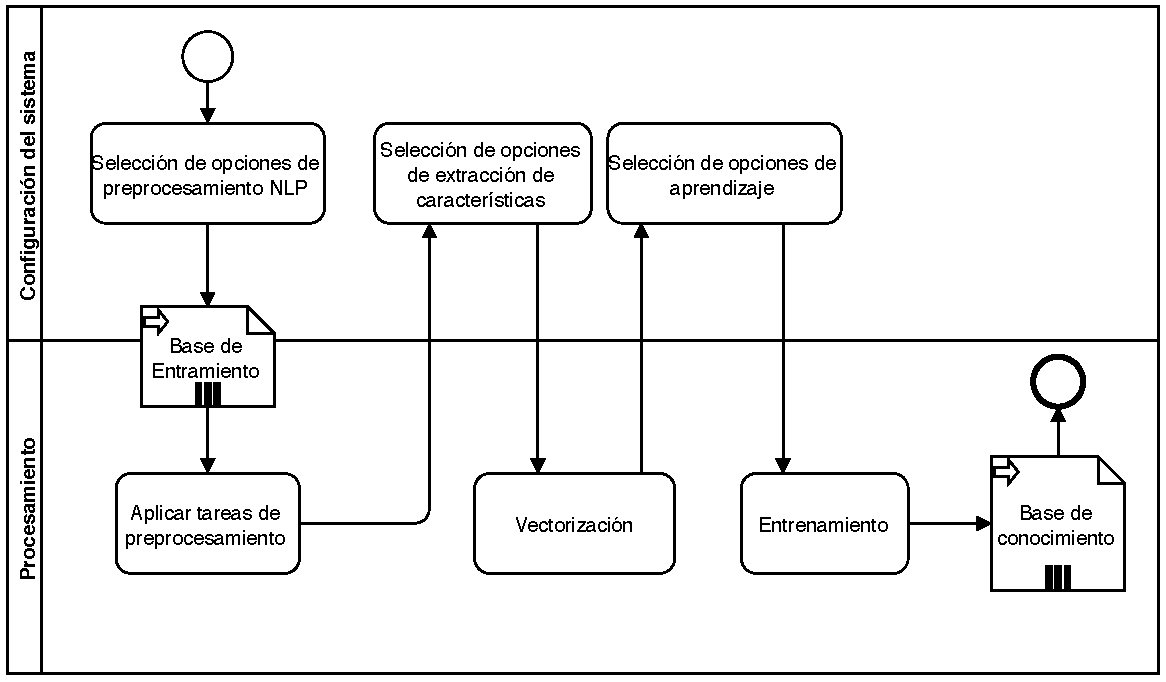
\includegraphics[width=\textwidth]{bpmn-entrenamiento}


\cleardoubleevenemptypage
\part{Conclusiones}
\label{part:conclusiones}

%!TEX root = pfc-memoria.tex
%!TEX encoding = UTF-8 Unicode

\chapter{Conclusiones}

\chapter{Trabajo futuro}

Posibles ampliaciones:

\begin{itemize}
\item Guardado y recuperación de la base de conocimiento entrenada.
\item Añadir más métodos de aprendizaje
\item Añadir más opciones de extracción de características
\item Permitir formato de ficheros TSV y CSV con mayor libertad en el número de columnas y tipos de datos
\end{itemize}


\cleardoubleevenemptypage
\part{Apéndices}
\label{part:apendices}
\appendix

%!TEX root = pfc-memoria.tex
%!TEX encoding = UTF-8 Unicode

\chapter{Manual de instalación}

\epigraph{``Tenemos que dejar de optimizar para programadores y comenzar a optimizar para usuarios.''}{\textsc{Jeff Atwood}}

En este capítulo se describe el procedimiento de instalación de la aplicación y las bibliotecas de las que depende.

\section{Instalación de prerrequisitos}

El primer conjunto de bibliotecas necesarias para instalar son:
\begin{enumerate}
\item El framework de desarrollo \nombrebf{Qt~5.5}
\item El intérprete \nombrebf{Python~3.4}
\end{enumerate}

\subsection{Qt~5.5}

Existen versiones de Qt~5.5 para Mac~OS~X, GNU/Linux y Windows (32 y 64 bit).
En la dirección oficial de descarga para la modalidad de software libre \url{https://www.qt.io/download-open-source/} se puede obtener el fichero de instalación. Se puede realizar una instalación offline u online, pero recomiendo usar el instalador offline ya que necesitamos instalar todos los componentes, incluidos los opcionales.

Proporciona un asistente de instalación de los que estamos acostumbrados, de siguiente-siguiente. Se recomienda usar la carpeta de instalación por defecto en el directorio de casa del usuario, en el caso de Mac~OS~X será \blackdirectory{/Users/USUARIO/Qt5.5.0}. También hace falta marcar la opción de instalación completa, incluido el paquete con el código fuente de Qt, para poder instalar PyQt5.

\begin{figure}[htbp]
\centering
\includegraphics[width=11.5cm]{qt-1}
\caption{Asistente de instalación de Qt~5.5: Página de bienvenida}
\label{fig:qt-1}
\end{figure}

\begin{figure}[htbp]
\centering
\includegraphics[width=11.5cm]{qt-2}
\caption{Selección de ruta de instalación de Qt}
\label{fig:qt-2}
\end{figure}

\begin{figure}[htbp]
\centering
\includegraphics[width=11.5cm]{qt-3}
\caption{Seleccionar todos los componentes para instalar}
\label{fig:qt-3}
\end{figure}

\begin{figure}[htbp]
\centering
\includegraphics[width=11.5cm]{qt-4}
\caption{Aceptación de licencia}
\label{fig:qt-4}
\end{figure}

\begin{figure}[htbp]
\centering
\includegraphics[width=11.5cm]{qt-5}
\caption{Inicio de instalación}
\label{fig:qt-5}
\end{figure}

\begin{figure}[htbp]
\centering
\includegraphics[width=11.5cm]{qt-6}
\caption{Progreso de instalación}
\label{fig:qt-6}
\end{figure}

\begin{figure}[htbp]
\centering
\includegraphics[width=11.5cm]{qt-7}
\caption{Instalación completada}
\label{fig:qt-7}
\end{figure}

\begin{figure}[htbp]
\centering
\includegraphics[width=11.5cm]{qt-8}
\caption{Finalización del asistente de instalación de Qt~5.5}
\label{fig:qt-8}
\end{figure}


\subsection{Python~3.4}

Python se encuentra actualmente en dos ``sabores'', versión 2 y versión 3, incompatibles entre sí. En este proyecto nos decantamos por usar el más moderno, y al momento de terminarse el proyecto, la versión concreta que se ha utilizado es Python~3.4.3, aunque debería funcionar en cualquier 3.4.x

Descargar la versión apropiada para su sistema operativo desde la dirección oficial \url{https://www.python.org/downloads/} y seguir las instrucciones del asistente de instalación o de las instrucciones de instalación de la documentación. En el caso de sistemas Mac~OS~X y Windows, se proporciona un asistente de instalación de los binarios; sin embargo para sistemas GNU/Linux se ofrece el paquete del código fuente de Python~3.4.3 listo para compilar.

Otra opción para usar en linux, es utilizar el intérprete Python de su distribución, si es que ésta proporciona alguna versión 3.4, incluyendo el módulo de entornos virtuales \path{venv} y el gestor de paquetes de Python \path{pip} (en Ubuntu son los paquetes \codet{python3-all-dev}, \codet{python3-venv} y \codet{python3-pip}).

\section{Instalación de bibliotecas}

A partir de este momento, tendremos disponibles en la consola el comando de Qt \path{qmake}, y los de Python \path{python3}, \path{pyvenv-3.4} y \path{pip3}.

Es necesario instalar los paquetes de desarrollo. En el caso de Mac~OS~X, la última versión de Xcode; y para Ubuntu, los paquetes listados en el \fullref{lst:ubuntu-apt-get}.

\begin{listing}[htbp]
\begin{minted}{bash}
$ sudo apt-get install ubuntu-dev-tools build-essential \
                       python3-all-dev python3-venv python3-pip \
                       xorg-dev libgl1-mesa-dev libglu1-mesa-dev \
                       libopenblas-dev
\end{minted}
\caption{Paquetes adicionales en Ubuntu}
\label{lst:ubuntu-apt-get}
\end{listing}

\FloatBarrier

Necesitamos las siguientes bibliotecas:
\begin{enumerate}
\item El generador de código \nombrebf{SIP} de Riverbank para la correcta compilación de PyQt5.
\item El \emph{binding} o adaptador de Qt5 para Python llamado \nombrebf{PyQt5} de Riverbank.
\item Los paquetes de pip listados en \blackdirectory{project/requirements.txt}
\end{enumerate}

Los programas de Riverbank pueden descargarse de la página oficial (se pueden probar con versiones futuras sin ningún miedo a perder la compatibilidad hacia atrás):
\begin{itemize}
\item \url{https://riverbankcomputing.com/software/pyqt/download5},\\
archivo \path{PyQt-gpl-5.5.tar.gz}
\item \url{https://www.riverbankcomputing.com/software/sip/download},\\
archivo \path{sip-4.16.9.tar.gz}
\end{itemize}

El primer paso es crear un entorno virtual de Python para evitar conflictos con otras aplicaciones en Python, como paso preventivo, y sin necesidad de tener permisos de superusuario (\autoref{lst:pyvenv}).

\begin{listing}[htbp]
\begin{minted}{bash}
$ pyvenv-3.4 --clear py34
$ source py34/bin/activate
(py34) $ pip3 install -U pip
\end{minted}
\caption[Creación del entorno virtual (pyvenv)]{Creación del entorno virtual (pyvenv), activación y actualización local de \path{pip}}
\label{lst:pyvenv}
\end{listing}
\FloatBarrier

Una vez completado, compilamos e instalamos \path{sip} (\autoref{lst:sip}).

\begin{listing}[htbp]
\begin{minted}{bash}
(py34) $ tar xzf sip-4.16.9.tar.gz
(py34) $ cd sip-4.16.9
(py34) $ python3.4 configure.py
(py34) $ make
(py34) $ make install
(py34) $ cd ..
\end{minted}
\caption{Compilación e instalación de SIP}
\label{lst:sip}
\end{listing}
\FloatBarrier

Después de la instalación de \path{sip}, procedemos a instalar el binding. Nos hemos encontrado un bug en Qt~5.5.0, y necesitamos aplicar un parche previo (\autoref{lst:parche}).

\begin{listing}[htbp]
\begin{minted}{diff}
--- PyQt-gpl-5.5/configure.py   2015-08-07 12:49:40.000000000 +0200
+++ PyQt-gpl-5.5/configure.py   2015-08-07 12:47:23.000000000 +0200
@@ -697,7 +697,7 @@
         lines = f.read().split('\n')
         f.close()
 
-        self.qt_licensee = lines[0]
+        self.qt_licensee = 'Open Source'
         self.qt_shared = (lines[1] == 'shared')
         self.pyqt_disabled_features = lines[2:-1]
 
\end{minted}
\caption[Corrección de bug en Qt~5.5.0]{Corrección de bug en Qt~5.5.0 (\path{PyQt-gpl-5.5-fix-license-typo.diff})}
\label{lst:parche}
\end{listing}
\FloatBarrier

\newpage
Configuramos e instalamos PyQt5 (\autoref{lst:pyqt5}).

\begin{listing}[htbp]
\begin{minted}{bash}
(py34) $ tar xzf PyQt-gpl-5.5.tar.gz
(py34) $ patch -p0 < PyQt-gpl-5.5-fix-license-typo.diff
(py34) $ cd PyQt-gpl-5.5
(py34) $ python3.4 configure.py --qmake ~/Qt5.5.0/5.5/*/bin/qmake
(py34) $ make
(py34) $ make install
(py34) $ cd ..
\end{minted}
\caption{Compilación e instalación de PyQt5}
\label{lst:pyqt5}
\end{listing}
\FloatBarrier

Como último paso, instalamos los paquetes listados como dependencias en el fichero \path{requirements.txt} (\autoref{lst:pip-requirements-txt}).

\begin{listing}[htbp]
\begin{minted}{bash}
(py34) $ pip3 install -U -r project/requirements.txt
(py34) $ python3.4 -m nltk.downloader all
\end{minted}
\caption{Instalación de paquetes de \codet{pip} de dependencias}.
\label{lst:pip-requirements-txt}
\end{listing}
\FloatBarrier

\section{Inicio del programa}

Para iniciar la ejecución del programa, se puede hacer como se indica en el \autoref{lst:start-pfcsamr}.

\begin{listing}[htbp]
\begin{minted}{bash}
(py34) $ cd project
(py34) $ PYTHONPATH=. pfcsamr/gui.py
\end{minted}
\caption{Inicio del programa}.
\label{lst:start-pfcsamr}
\end{listing}
\FloatBarrier


\chapter{Manual de usuario}

\epigraph{``Los ordenadores son buenos siguiendo instrucciones, no leyendo tu mente.''}{\textsc{Donald Knuth} (1938--)}

\section{Carga del fichero de entrenamiento}

La primera pantalla que se muestra al abrir la aplicación es la pestaña de carga (\autoref{fig:ss-01-load-tab}).

\begin{figure}[H]
\centering
\includegraphics[width=13cm]{ss-01-load-tab}
\caption{Pantalla de carga del fichero de entrenamiento}
\label{fig:ss-01-load-tab}
\end{figure}

\newpage
Al pulsar sobre el botón \menu{Select file} aparece un cuadro de diálogo que permite seleccionar el fichero \path{train.tsv} de entrenamiento (\autoref{fig:ss-02-load-file}).

\begin{figure}[H]
\centering
\includegraphics[width=14cm]{ss-02-load-file}
\caption{Pantalla de selección del fichero de entrenamiento}
\label{fig:ss-02-load-file}
\end{figure}

\newpage
Una vez seleccionado, marcar la opción de carga parcial si se desea, indicando el número de muestras. A continuación, pulsar el botón \menu{LOAD}, con lo que aparece el fichero en forma de tabla en el panel de datos (\autoref{fig:ss-03-file-loaded}).

\begin{figure}[H]
\centering
\includegraphics[width=14cm]{ss-03-file-loaded}
\caption{Pantalla con el fichero de entrenamiento cargado}
\label{fig:ss-03-file-loaded}
\end{figure}

\newpage
\section{Opciones de preprocesamiento de texto}
\label{sec:manual-preproc}

Una vez cargado, pasamos a la siguiente pestaña de opciones de preprocesamiento. En esta pantalla, marcamos las opciones deseadas, y a continuación pulsamos el botón \menu{RUN} para proceder al preprocesamiento. Se muestra una barra de progreso a la derecha de la barra de estado, y al terminar, se actualiza el panel de datos con las muestras preprocesadas (\autoref{fig:ss-04-preproc-tab}).

\begin{figure}[H]
\centering
\includegraphics[width=14cm]{ss-04-preproc-tab}
\caption{Pantalla de opciones de preprocesamiento}
\label{fig:ss-04-preproc-tab}
\end{figure}

\newpage
\section{Extracción de características}
\label{sec:manual-features}

El siguiente paso es la extracción de características. Pulsar en la pestaña y marcar las opciones deseadas para la extracción de n-gramas y su reducción. Pulsar en el botón \menu{RUN} para proceder con la transformación. Al finalizar, se muestra el panel de datos con una característica en cada columna, y su valor para cada muestra. El encabezado de la columna indica el n-grama concreto (\autoref{fig:ss-05-feat-tab}).

\begin{figure}[H]
\centering
\includegraphics[width=14cm]{ss-05-feat-tab}
\caption{Pantalla de opciones de extracción de características}
\label{fig:ss-05-feat-tab}
\end{figure}

\newpage
\section{Aprendizaje automático del modelo}
\label{sec:manual-learn}

A continuación, avanzamos de pestaña para las opciones de aprendizaje. Se recomienda dejar marcado la división del conjunto en subconjunto de entrenamiento y subconjunto de autoevaluación, para poder obtener una puntuación del modelo aprendido.

Elegir el modelo concreto en la segunda fila de pestañas y pulsar el botón \menu{RUN}. Cuando finalice el aprendizaje, se actualizará el valor de la puntuación (etiqueta \codet{SCORE: }). Hay cinco modelos a elegir, no es obligatorio entrenarlos todos, pero está bien hacerlo para comparar su puntuación y elegir el mejor.

Se puede repetir tantas veces como se desee e ir alterando los parámetros para encontrar la mayor puntuación (\autoref{fig:ss-06-learn-tab}).

\begin{figure}[H]
\centering
\includegraphics[width=14cm]{ss-06-learn-tab}
\caption{Pantalla de aprendizaje (\codep{MultinomialNB})}
\label{fig:ss-06-learn-tab}
\end{figure}

\newpage
\section{Clasificación del conjunto de clasificación}

Una vez entrenado alguno de los modelos, avanzar pulsando la pestaña siguiente (\autoref{fig:ss-07-classify-tab}). Pulsar el botón \menu{Select file} para elegir el fichero \path{test.tsv} de evaluación.

\begin{figure}[H]
\centering
\includegraphics[width=14cm]{ss-07-classify-tab}
\caption{Pantalla de la pestaña de clasificación}
\label{fig:ss-07-classify-tab}
\end{figure}

\newpage
Se puede activar la opción de carga parcial e indicar el número de muestras, si se desea. A continuación pulsar \menu{LOAD} para realizar la carga y la visualización en el panel de datos (\autoref{fig:ss-08-classify-test-loaded}).

\begin{figure}[H]
\centering
\includegraphics[width=14cm]{ss-08-classify-test-loaded}
\caption{Pantalla con el conjunto de clasificación cargado}
\label{fig:ss-08-classify-test-loaded}
\end{figure}

\newpage
Pulsando el botón \menu{1. PREPROCESS} se realiza el preprocesamiento de texto de clasificación de manera análoga a como se preprocesó el texto de entrenamiento en la fase de entrenamiento (\autoref{sec:manual-preproc}). Se actualizará el panel de datos con el resultado (\autoref{fig:ss-08-classify-test-loaded}).

\begin{figure}[H]
\centering
\includegraphics[width=14cm]{ss-09-classify-test-preproccesed}
\caption{Pantalla con el texto preprocesado}
\label{fig:ss-09-classify-test-preproccesed}
\end{figure}

\newpage
Siguiendo con el procedimiento, pulsamos el botón \menu{2. FEATURES} para extraer las características del texto de clasificación preprocesado, que se realiza automáticamente de manera análoga a como se hizo en la fase de entrenamiento (\autoref{sec:manual-features}). Al terminar, se muestra en el panel de datos las características de las muestras a clasificar (\autoref{fig:ss-10-classify-test-featured}).

\begin{figure}[H]
\centering
\includegraphics[width=14cm]{ss-10-classify-test-featured}
\caption{Pantalla de características}
\label{fig:ss-10-classify-test-featured}
\end{figure}


\newpage
El último paso es realizar las predicciones. Para ello, elija un modelo del cuadro desplegable. Este modelo debería haber sido entrenado previamente en el paso de entrenamiento (\autoref{sec:manual-learn}), en caso contrario se mostrará un error. Pulsar el botón \menu{3. CLASSIFY} para clasificar las muestras. Aparecerá en el panel de datos las muestras originales con una columna añadida del sentimiento predicho por el modelo seleccionado (\autoref{fig:ss-11-classify-test-predictions}). Si se desea, se puede repetir usando otro modelo.

\begin{figure}[H]
\centering
\includegraphics[width=14cm]{ss-11-classify-test-predictions}
\caption{Pantalla con las predicciones de sentimiento}
\label{fig:ss-11-classify-test-predictions}
\end{figure}

Posteriormente, pulsando el botón \menu{Save file for submission to kaggle} se puede guardar el resultado de la clasificación en el formato \path{.csv} para posteriormente entregar en Kaggle.\footnote{\url{https://www.kaggle.com/c/sentiment-analysis-on-movie-reviews}}

\newpage
En cualquier momento, se puede usar el menú \menu{File} para reiniciar el sistema, o abrir o guardar las opciones de la sesión para reanudar posteriormente.

\begin{figure}[H]
\centering
\includegraphics[width=\textwidth]{ss-12-menu-file}
\caption[Pantalla con el menú \codet{FILE}]{Pantalla con el menú \menu{File}}
\label{fig:ss-12-menu-file}
\end{figure}




%% %% %% %% %% %% %%

\backmatter

%% biliografía %%
\nocite{*}
\printbibliography[heading=bibintoc,title=\bibname]

%% índices y tablas %

\cleardoublepage
\addcontentsline{toc}{chapter}{Listado de listings}
\listoflistings

\cleardoublepage
\addcontentsline{toc}{chapter}{Índice alfabetico}
\printindex

\end{document}
